\documentclass[10pt, a4paper]{article}
\usepackage{lrec2016}
%% \usepackage{multibib}
%% \newcites{languageresource}{Language Resources}
\usepackage{graphicx}
\usepackage{url}
\usepackage{xspace}
\usepackage{multirow}
% for eps graphics

\usepackage{epstopdf}
\usepackage[latin1]{inputenc}
 
\newcommand{\secref}[2][]{Section#1~\ref{#2}\xspace}
\newcommand{\tabref}[2][]{Table#1~\ref{#2}\xspace}
\newcommand{\figref}[2][]{Figure~\ref{#2}#1\xspace}
\newcommand{\eqnref}[2][]{Equation~\ref{#2}#1\xspace}

\newcommand{\spadeaff}{\ensuremath{\spadesuit}\xspace}
\newcommand{\heartaff}{\ensuremath{\heartsuit}\xspace}
\newcommand{\diamondaff}{\ensuremath{\diamondsuit}\xspace}
\newcommand{\clubaff}{\ensuremath{\clubsuit}\xspace}


% Use cmtt for typewriter font -- narrower, fits better on page
\renewcommand{\ttdefault}{cmtt}

\title{Classifying Out-of-vocabulary Terms in a Domain-Specific Social
  Media Corpus}

\name{SoHyun Park,$^{\clubaff}$ Afsaneh Fazly,$^{\diamondaff}$ Annie Lee,$^{\diamondaff}$ Brandon Seibel,$^{\diamondaff}$ Wenjie
  Zi$^{\diamondaff}$ and Paul Cook$^{\clubaff}$}

\address{$\clubaff$ Faculty of Computer Science, University of New Brunswick\\
$\diamondaff$ VerticalScope, Toronto Canada\\
\url{sohyun.park@unb.ca},
\url{{afazly,alee,bseibel,wzi}@verticalscope.com},
\url{paul.cook@unb.ca}\\}

%% \url{alee@verticalscope.com}
%% \url{bseibel@verticalscope.com}
%% \url{wzi@verticalscope.com}

\abstract{In this paper we consider the problem of out-of-vocabulary
  term classification in web forum text from the automotive domain. We
  develop a set of nine domain- and application-specific categories
  for out-of-vocabulary terms. We then propose a supervised approach
  to classify out-of-vocabulary terms according to these categories,
  drawing on features based on word embeddings, and linguistic
  knowledge of common properties of out-of-vocabulary terms. We show
  that the features based on word embeddings are particularly
  informative for this task. The categories that we predict could
  serve as a preliminary, automatically-generated source of lexical
  knowledge about out-of-vocabulary terms. Furthermore, we show that
  this approach can be adapted to give a semi-automated method for
  identifying out-of-vocabulary terms of a particular category,
  automotive named entities, that is of particular interest to us.  \\
%% Each article must include an abstract of 150 to 200 words in Times
%% 9 pt with interlinear spacing of 10 pt. The heading Abstract should be
%% centred, font Times 10 bold. This short abstract will also be used for
%% printing a Booklet of Abstracts containing the abstracts of all papers
%% presented at the Conference. \\ 
\newline 
\Keywords{Lexical acquisition, social media text, out-of-vocabulary words}}

\begin{document}

\maketitleabstract

\section{Domain-specific OOV Classification}

Out-of-vocabulary terms are more common in social media text than
more-conventional text types \cite{Baldwin+:2013a}.
%% Social media text contains a much higher proportion of
%% out-of-vocabulary terms than more-conventional text
%% \cite{Baldwin+:2013a}. 
Moreover, many domain-specific technical terms
are not included in general-purpose dictionaries and lexical
resources. Domain-specific social media corpora are therefore
particularly rife with out-of-vocabulary terms.

Many natural language processing (NLP) systems for tasks including
sentiment analysis and question answering rely on lexical
knowledge. In the case that a text being processed contains
out-of-vocabulary terms, system performance suffers because lexical
knowledge is not available for these words. Much research in NLP has
therefore focused on lexical acquisition --- automatically learning
syntactic or semantic properties of words from corpora
\cite[for example]{Hearst1992,Lin1998,Turney2003}.


%% VerticalScope owns many web forums, including in particular several
%% in the automotive domain. VerticalScope has a business interest in
%% being able to more-intelligently analyze this text. 
%% In this work we focus specifically on out-of-vocabulary (OOV) terms in
%% web forum text from the automotive domain. 

In this work we focus specifically on out-of-vocabulary (OOV) terms in
web forum text from the automotive domain. The focus on the automotive
domain is motivated by the business interests of VerticalScope,
Inc.\ (the industrial collaborator in this research) in being able to
more-intelligently analyze this text. VerticalScope, Inc.\ is a
Canadian company that owns and operates one of the most highly visited
automotive networks of online forums. The goal of this research is to
automatically classify OOVs as one of a predefined set of domain- and
application- specific categories --- e.g., automotive named entity
(NE), slang, spelling error, foreign term. This automatically-inferred
coarse-grained lexical knowledge will later be used to build
vocabularies focused on, or excluding, particular types of expressions
in an effort to improve topic models \cite[for example]{Blei2003} of
automotive web forum text to better understand its contents. This
knowledge will also be leveraged in an effort to improve downstream
NLP tasks, such as named entity recognition, for this specialized text
type.


\section{OOVs in Automotive Social Media}


%% Here is how I picked the sample: this is a random selection of all
%% alphanumeric OOVs (that do not appear in a large english
%% dictionary, nor in our list of terms from freebase make/models),
%% that are more frequent than 1000 (in our 2013--2014 collection),
%% and are between 2 and 10 in length.


For this study, we focused on a random sample of 665 alphanumeric OOVs
that 1.) have frequency greater than 1000 in an automotive web forum
corpus of roughly 150 million posts from the years 2013 and 2014; 2.)
consist of two to ten characters; 3.) do not occur in any of the GNU
Aspell English Dictionary version
0.7,\footnote{\url{http://aspell.net/}} a list of automotive terms
from Freebase,\footnote{\url{https://www.freebase.com/}} or a list of
automotive acronyms.

These OOVs were manually annotated by a single judge as one of nine
OOV categories, described in \tabref{tbl:categories}. The categories
were determined based on the common types of OOVs found in this
data. The annotator was a computational linguist with knowledge of the
automotive domain, who was not otherwise involved in building the
automatic OOV classification system.

A sample of twenty items was also annotated by a second judge, also an
author of this paper, who in this case was directly involved in
building the automatic OOV classification system. The observed
agreement and unweighted Kappa were, 0.65 and 0.55, respectively. We
are, however, particularly interested in the \textsc{ne-auto}
class. These terms include car makes, models, and trims (e.g.,
\emph{XLT} in \emph{Ford F-150 XLT}), that are not listed in any of the
lexical resources considered. Because of the relatively low
inter-annotator agreement on the nine-way annotation task, we
therefore also considered a two-way annotation task for the categories
\textsc{ne-auto} and ``other'' (i.e., the eight other classes). Here
the observed agreement and unweighted Kappa were 0.90 and 0.78,
respectively, suggesting that human annotators can much more reliably
distinguish these two categories than the full set of nine categories.


\begin{table*}
\begin{center}
\begin{tabular}{lcll}

 Category & Num.\ items & Explanation & Examples \\ \hline

 \textsc{auto} & 45 & Automotive terms (not NEs) & \emph{defuel}, \emph{rebalance} \\

 \textsc{drug} & 95 & Drug names & \emph{levoxyl}, \emph{nexium} \\

 \textsc{foreign} & 47 &  Non-English terms & \emph{rezeptfrei}, \emph{depuis}\\%, \emph{mucho} \\

 \textsc{measurement}& 58 & Units of measurement & \emph{77k}, \emph{100mph} \\

 \textsc{ne-auto}& 140~\, & Automotive-related NEs & \emph{ls3}, \emph{volks} \\
% ls3 is a Chevrolet engine name

 \textsc{ne-other}& 41& Non-automotive NEs & \emph{blackhawks}, \emph{diaz} \\

 \textsc{noise} & 87  & Noise, and items that don't fit other
 categories & \emph{kagvjfcjfx}, \emph{kzvddzfv52} \\

 \textsc{slang}& 59 & Internet slang and non-standard forms & \emph{heyyaa}, \emph{lol2}\\ %, \emph{ceos} \\

 \textsc{spelling-error}& 93 & Spelling errors & \emph{youll}, \emph{genericfor} \\

\end{tabular}
\caption{The categories of OOVs, along with an explanation of, and
  examples of, each.\label{tbl:categories}}
\end{center}
\end{table*}

\section{Model}

%% ***** Reviewer #3 comment: have a better knowledge about the
%% effects of tokenization; potential markers left out by tokenization
%% processes are sometimes useful to identify OOVs (e.g.  quotation
%% marks around words perceived as neologisms or unusual by he
%% writer);
%% 
%% We didn't look at features like this because many of the words do
%% not seem to be neologisms in the contexts in which they are used
%% (i.e., they're just regular words within these communities). *****

%% ***** Reviewer #3: have an insight on how apparent compounds were
%% treated and whether hyphenated words were given special attention
%% (variants due to out of place hyphenation, compounds that are made
%% of two recognizable words but taken as an OOV if analyzed as a
%% whole).

In this preliminary work we consider a supervised approach to OOV
classification using the following classes of features.

\subsection{Character $N$-grams}

Certain character $n$-grams are more frequent in some categories than
others. For example, spelling errors and non-standard social media
forms contain character sequences that are uncommon in standard
English due to character deletion or repetition. In drug names,
character sequences such as word-final $ne$ and $an$ (e.g., as in
\emph{ketamine} and \emph{niaspan}) are particularly common. Character
$n$-grams are often applied in language identification \cite[for
  example]{LuiBaldwin2011} and could therefore be particularly
informative for identifying foreign terms. Our first set of features
therefore consists of the character $n$-grams in a given OOV, for $n =
1$--$3$.

\subsection{Character $N$-gram Models}

Many \textsc{ne-auto} OOVs contain character sequences that are rare
in standard English (e.g., \emph{ls2} an engine model name). Moreover,
many \textsc{foreign} OOVs contain character sequences that are
uncommon in English. We construct character-level bigram and trigram
models from corpora of English, German, and Spanish. For English we
used the Brown Corpus \cite{Francis1979}, while for German and Spanish
we used the corresponding versions of the Universal Declaration of
Human Rights available through NLTK \cite{Bird2009}. We also built
language models for a list of automotive acronyms, and a list of
automotive terms from Freebase. For these features, for a given OOV,
we calculate its probability under each of these bigram and trigram
language models.


\subsection{Frequency\label{sec:features:frequency}}

We hypothesize that categories such as \textsc{slang} and
\textsc{spelling-error} will tend to be infrequent in well-edited
text, and relatively frequent in text types such as social media
text. Moreover, categories such as \textsc{ne-auto} and \textsc{auto}
will tend to be relatively frequent in text from that domain ---
whether social media text or not --- and relatively infrequent in
other domains. We obtain corpora corresponding to a variety of text
types (described in \secref{sec:corpora} below). For these features,
for a given OOV, we calculate its frequency in each corpus normalized
by the total number of tokens in the corresponding corpus.

\subsection{Word Embeddings\label{sec:features:embeddings}}

Word embeddings (e.g., word2vec, Mikolov et al., 2013) are vector
representations of words that capture aspects of their syntax and
semantics. We hypothesize that the embedding for a given OOV will tend
to be close in vector space to OOVs of the same category. For this
feature set, we run word2vec on a corpus of web forum text (described
in \secref{sec:corpora} below), and use the resulting embedding for a
given OOV as a feature vector. In the case that an OOV does not have a
word embedding (which happens when the OOV does not occur in the
corpus, or when it does occur in the corpus but has frequency below a
threshold), we represent it as the average of the vectors for all
other OOVs that do have word embeddings.


%% Liz: What do we do in the event that we don't have a vector for an
%% OOV?  

We use the following settings for word2vec: the skipgram model, a
vector dimensionality of 200, a window size of 5, and a minimum
frequency of 10. To select these parameters, we trained word2vec with
a variety of parameter settings for the model (skipgram and cbow),
number of dimensions, and window size. We evaluated the vectors
obtained on the analogy task of Mikolov et
al.\ \shortcite{Mikolov+:2013}; the selected parameters gave the best
results on this task.

%% Hi Professor,

%% Sorry for the late response! Here is the list of parameter setting combinations I considered:

%% 1) negative=20, skip-gram, size=200, sample=0(default), window=5(default) - 31% accuracy

%% 2) negative=20, skip-gram, size=500, sample=1e-5, windows=5(default) - 27% accuracy

%% 3) negative=20, cbow, size=500, sample=1e-5, window=5(default) -25% accuracy

%% 4) negative=20, cbow, size=200, sample=1e-5, window=5(default) -22.9% accuracy

%% 5) negative=20, skip-gram, size=300, sample=1e-5, windows=5(default) -25.1% accuracy

%% 6) negative=20, cbow, size=300, sample=1e-5, window=5(default) -24.7% accuracy

%% 7) negative=20, skip-gram, size=200, sample=0(default), window=1 -34%

%% 8) negative=20, skip-gram, size=200, sample=0(default), window=5 -32%

%% Thank you,
%% Liz Park


\subsection{Surface Form}

We introduce five further features based on observed properties of the
surface forms of OOVs.

\begin{itemize}

\item We observe that many OOVs in the \textsc{slang} and
  \textsc{spelling-error} categories appear to be formed by
  concatenating two in-vocabulary words (e.g., \emph{eachother}, a
  spelling error, is formed from \emph{each} and \emph{other}). The
  first surface form feature is a binary feature that takes the value
  1 if a given OOV can be split into a prefix and suffix that each
  occur in a dictionary (the GNU Aspell English Dictionary), and 0
  otherwise.

\item Many OOVs in the \textsc{noise} and \textsc{measurement}
  categories are relatively shorter than items in the other
  categories. We hypothesize that word length could be informative of
  categories of OOVs. The second surface form feature corresponds to
  the number of characters in a given OOV.

\item We observe many OOVs that consist of a combination of letters
  and digits in the categories \textsc{noise} (e.g., \emph{w43y5h6}),
  \textsc{slang} (e.g., \emph{high5}), and \textsc{ne-auto} (e.g.,
  \emph{m8000}). The third surface form feature feature represents the
  wordshape of a given OOV. Contiguous sequences of consonants,
  vowels, and digits are mapped to the symbols \emph{c}, \emph{v}, and
  \emph{d}, respectively. For example, \emph{high5} is represented as
  \emph{cvcd}.

\item We note many OOVs in \textsc{noise}, \textsc{slang}, and
  \textsc{spelling-error} that have many repeated letters, such as
  \emph{mmm} and \emph{loong}. The fourth surface form feature
  represents whether a given OOV contains two consecutive repeated
  characters.

\item Many spelling errors are within a small edit distance (often one
  or two) of their correction. The minimum of the edit distance
  between an OOV and any in-vocabulary word could therefore be
  particularly informative as to whether that OOV is a
  \textsc{spelling-error}. For the final surface form feature we
  calculate the minimum edit distance between a given OOV and any word
  in a dictionary (again, GNU Aspell).

\end{itemize}

\section{Materials and Methods}


\subsection{Corpora\label{sec:corpora}}


Three corpora were used for this research: 

\begin{description}
\item[Forum] Posts from a variety of English web forums such as
  \url{talkford.com}, \url{watchfreeks.com}, and
  \url{samsunggalaxyreviews.com} corresponding to verticals such as
  automotive, collectibles, and technology.
\item[Wikipedia] A dump of English Wikipedia from 1 September 2015.
\item[Twitter] A sample of English tweets collected from the Twitter
  Streaming APIs\footnote{\url{https://dev.twitter.com/}} from
  November 2014 to March 2015.
\end{description}

%%  Tool used for metadata removal for each corpus:
%% 		Wiki: WikiExtractor from https://github.com/attardi/wikiextractor
%% 		Twitter: Didn't use any tool for this corpus.
%%		Forum: Scala code provided by VS

\noindent
The Wikipedia corpus was pre-processed to remove meta-data, such as
wiki markup, using
WikiExtractor.\footnote{\url{https://github.com/attardi/wikiextractor}}
The forum corpus was similarly pre-processed to remove forum tags.
The Wikipedia corpus was tokenized using the Stanford CoreNLP
tokenizer \cite{Manning+:2014}. The forum and Twitter corpora were
tokenized using a tokenizer developed for tweets, adapted from
\cite{OConnor+:2010}. \tabref{tbl:corpora} shows the number of
documents, tokens, and OOVs from our dataset, in each corpus.\\

These corpora were used to calculate the frequency features
(\secref{sec:features:frequency}). The forums corpus was used for
training word2vec to calculate the word embeddings features
(\secref{sec:features:embeddings}).

\begin{table}
\begin{center}
\begin{tabular}{lccc}
\multirow{2}{*}{Corpus}&\multirow{2}{*}{Num.\ docs}&\multirow{2}{*}{Num.\ tokens} &Num.\ OOVs\\ 
& & & from dataset \\
 \hline
Wikipedia&4.9M&1.7B&340\\
Twitter&98.9M&1.2B&474\\
Forums&80.0M&5.0B&657\\
\end{tabular}
\end{center}
\caption{The number of documents, tokens, and OOVs from our dataset,
  in each corpus.
\label{tbl:corpora}}
\end{table}

\subsection{Experimental Setup}

10x10-fold stratified cross-validation experiments were carried out on
the dataset of OOVs using the features described above with a maximum
entropy classifier.\footnote{We also considered random forests, a
  linear support vector machine (SVM), and an SVM using a radial basis
  function kernel, however, we saw little difference in results, and
  so only describe and report results for maximum entropy here.} We
considered both a nine-way classification task (i.e., classifying OOVs
according to the categories in \tabref{tbl:categories}) and a two-way
classification task for the classes \textsc{ne-auto} and ``other''
(i.e., the remaining eight categories). We considered each feature set
on its own, as well as combinations of feature sets.  For each
experiment we calculated macro-averaged precision, recall, and
F1 score, as well as accuracy. As a point of comparison, we further
considered a most-frequent class baseline.

\section{Experimental Results}

Macro-averaged precision, recall, and F1 score, as well as accuracy,
are shown in \tabref{tbl:results} for the most-frequent class
baseline, each feature set individually, all feature sets combined,
and ablative experiments in which we consider all-but-1 feature set,
for each feature set, for the nine-way classification task.

The character $n$-gram, word embedding, and surface form features all
substantially outperform the baseline, in terms of all evaluation
metrics, while the character $n$-gram models and frequency features
perform on par with the baseline. This suggests that character
$n$-grams in OOVs, distributional information captured by word
embeddings, and the linguistic knowledge captured by the surface form
features are all highly informative for OOV classification in
automotive web forum text. In future work we intend to explore the use
of additional corpora, in particular domain-specific texts from
non-social media text types, to further explore the impact of
frequency in OOV classification.

The combination of all features (shown as [A+B+C+D+E] in
\tabref{tbl:results}) performs roughly on par with the best individual
feature set, the word embeddings. We further explore combinations of
features in ablative experiments, in which we consider all feature
sets but one, holding out each feature set in turn.

The classifier using all feature sets except the frequency features
([A+B+D+E] in \tabref{tbl:results}) performs best in terms of all
evaluation metrics. That these features (all feature sets excluding
the frequency features) improve over any individual feature set
indicates that they carry complementary information about OOV
categories. Moreover, this further suggests that the frequency
features do not carry information about OOV categories as they are
currently formulated.  The relatively low performance when the word
embedding features are omitted ([A+B+C+E] in \tabref{tbl:results})
reinforces the power of these features for this task.


%% ***** PC: Do I want to bother doing this??? I could do a binomial
%% test. I'm not sure about applying McNemar to multi-class
%% data. Could do chi-square or binomial test.



\begin{table*}
\begin{center}
\begin{tabular}{lcccc}

\textbf{Method}& \textbf{Precision}&\textbf{Recall}
&\textbf{F1 score}&\textbf{Accuracy}\\
 \hline
Most-frequent class baseline & 0.023 & 0.111 & 0.039 & 0.211 \\

\hline

[A] Characater $n$-grams (1-3) & 0.390 & 0.373 & 0.380 & 0.413\\

[B] Character $n$-gram models & 0.023 & 0.111 & 0.039 & 0.211 \\

[C] Frequency & 0.023 & 0.111 & 0.039 & 0.211 \\

[D] Word embeddings & 0.649 & 0.599 & 0.622 & 0.643 \\

[E] Surface form & 0.390 & 0.400 & 0.394 & 0.446 \\ 

[A+B+C+D+E] & 0.643 & 0.603 & 0.622 & 0.649 \\

[B+C+D+E] & 0.649 & 0.602 & 0.624 & 0.646 \\

[A+C+D+E] & 0.640 & 0.605 & 0.622 & 0.648 \\

[A+B+D+E] & \textbf{0.650} & \textbf{0.609} & \textbf{0.628} & \textbf{0.654} \\

[A+B+C+E] & 0.429 & 0.422 & 0.424 & 0.469 \\

[A+B+C+D] & 0.614 & 0.582 & 0.597 & 0.629 \\
\end{tabular}
\caption{Macro-averaged precision, recall, and F1 score, as well as
  accuracy, for the baseline, each feature set, and combinations of
  features for the nine-way classification task.\label{tbl:results}}
\end{center}
\end{table*}

We now consider precision, recall, and F1 score for each class, using
the best-performing features for the nine way classification task (all
feature sets except the frequency features, i.e., [A+B+D+E]). Results
are shown in \tabref{tbl:results-class}. The F1 scores for
\textsc{drug} and \textsc{measurement}, 0.892 and 0.843, respectively,
are relatively high. We are, however, particularly interested in
\textsc{ne-auto}, because of our need to identify automotive named
entities (such as car makes and models) that are not in our current
resources. Here the F1 score is somewhat lower, 0.703, with a
precision and recall of 0.633 and 0.802, respectively.

\begin{table}
\begin{center}
\begin{tabular}{lcccc}

\textbf{Method}& \textbf{Precision}&\textbf{Recall}
&\textbf{F1 score}\\
\hline

\textsc{domain-term} & 0.586 & 0.459 & 0.489 \\

\textsc{drug} & 0.899 & 0.945 &  0.892 \\

\textsc{foreign} & 0.675 & 0.744 &  0.673\\

\textsc{measurement} & 0.903 & 0.883 & 0.843 \\

\textsc{ne-other} & 0.466 & 0.200 & 0.367 \\ 

\textsc{ne-auto} & 0.633 & 0.802 & 0.703 \\

\textsc{noise} & 0.727 & 0.610 & 0.645 \\

\textsc{slang} & 0.468 & 0.433 & 0.462 \\

\textsc{spelling-error} & 0.524 & 0.499 &  0.502 \\

\end{tabular}
\caption{Precision, recall, and F1 score, for each class in the
  nine-way classification task, using the best performing feature
  combination from \tabref{tbl:results}.\label{tbl:results-class}}
%% Feature sets: ABDE
\end{center}
\end{table}

We now consider whether we can improve performance on \textsc{ne-auto}
by re-formulating the classification task as a 2-way task. Here we
consider a two-way classification task for \textsc{ne-auto} vs
\textsc{other}, i.e., all other classes. Results are shown in
\tabref{tbl:results2way}. In this case the most-frequent class is
\textsc{other}. As such, the most-frequent class baseline achieves a
precision, recall, and F1 score of 0 because no items are classified
as \textsc{ne-auto}. The word embeddings are again the best of the
individual feature sets in terms of recall, F1 score and
accuracy. However, in this case the surface form features achieve the
highest precision. The best F1 score for the two-way task is achieved
using all feature sets except the character $n$-gram features
([B+C+D+E] in \tabref{tbl:results2way}). In this case the F1 score
(0.676) is somewhat lower than the F1 score for the \textsc{ne-auto}
class using the best overall features for the nine-way task (0.703,
\tabref{tbl:results-class}). However, there is a precision--recall
trade-off. The precision for \textsc{ne-auto} for the best overall
features for the two-way task (0.725) is higher than that for the
nine-way task (0.633, \tabref{tbl:results-class}), although the recall
is lower (0.644 vs. 0.802).



\begin{table*}
\begin{center}
\begin{tabular}{lcccc}

\textbf{Method}& \textbf{Precision}&\textbf{Recall}
&\textbf{F1 score}&\textbf{Accuracy}\\
 \hline
Most-frequent class baseline & 0.000 & 0.000  & 0.000 & 0.789 \\

\hline

[A] Characater $n$-grams (1-3) & 0.499 & 0.222 & 0.292 & 0.788 \\

[B] Character $n$-gram models &  0.000 & 0.000 & 0.000 & 0.786 \\

[C] Frequency & 0.000 & 0.000 & 0.000 & 0.789 \\

[D] Word embeddings & 0.714 & 0.619 & 0.656 & 0.862 \\

[E] Surface form & \textbf{0.775} & 0.154 & 0.288 & 0.814 \\ 

[A+B+C+D+E] & 0.734 & 0.583 & 0.609 & 0.866 \\

[B+C+D+E] & 0.725 & \textbf{0.644} & \textbf{0.676} &  \textbf{0.873} \\

[A+C+D+E] & 0.741 & 0.586 & 0.618 & 0.867 \\

[A+B+D+E] & 0.735 & 0.567 & 0.615 & 0.869 \\

[A+B+C+E] & 0.510 & 0.257 & 0.332 & 0.793 \\

[A+B+C+D] & 0.728 & 0.557 & 0.586 & 0.863 \\
\end{tabular}
\caption{Precision, recall, and F1 score, for the \textsc{ne-auto}
  class, as well as accuracy, for the baseline, each feature set, and
  combinations of features, for the two-way classification
  task.\label{tbl:results2way}}
\end{center}
\end{table*}

We further consider precision and recall for the two-way classifier by
examining a precision--recall curve. For the two-way classifier using
all features except the character $n$-grams, we rank all items in the
dataset by the probability of the \textsc{ne-auto} class. The
precision--recall curve is shown in \figref{fig:pr}. Precision remains
relatively high, roughly 0.8, for recall values up to 0.5. This
suggests that this ranking could be useful for semi-automatic
identification of \textsc{ne-auto} terms, where lexicographers could
further analyze highly-ranked items.


\begin{figure}
\begin{center}
%% \includegraphics[scale=0.22]{pr-trimmed.png} 
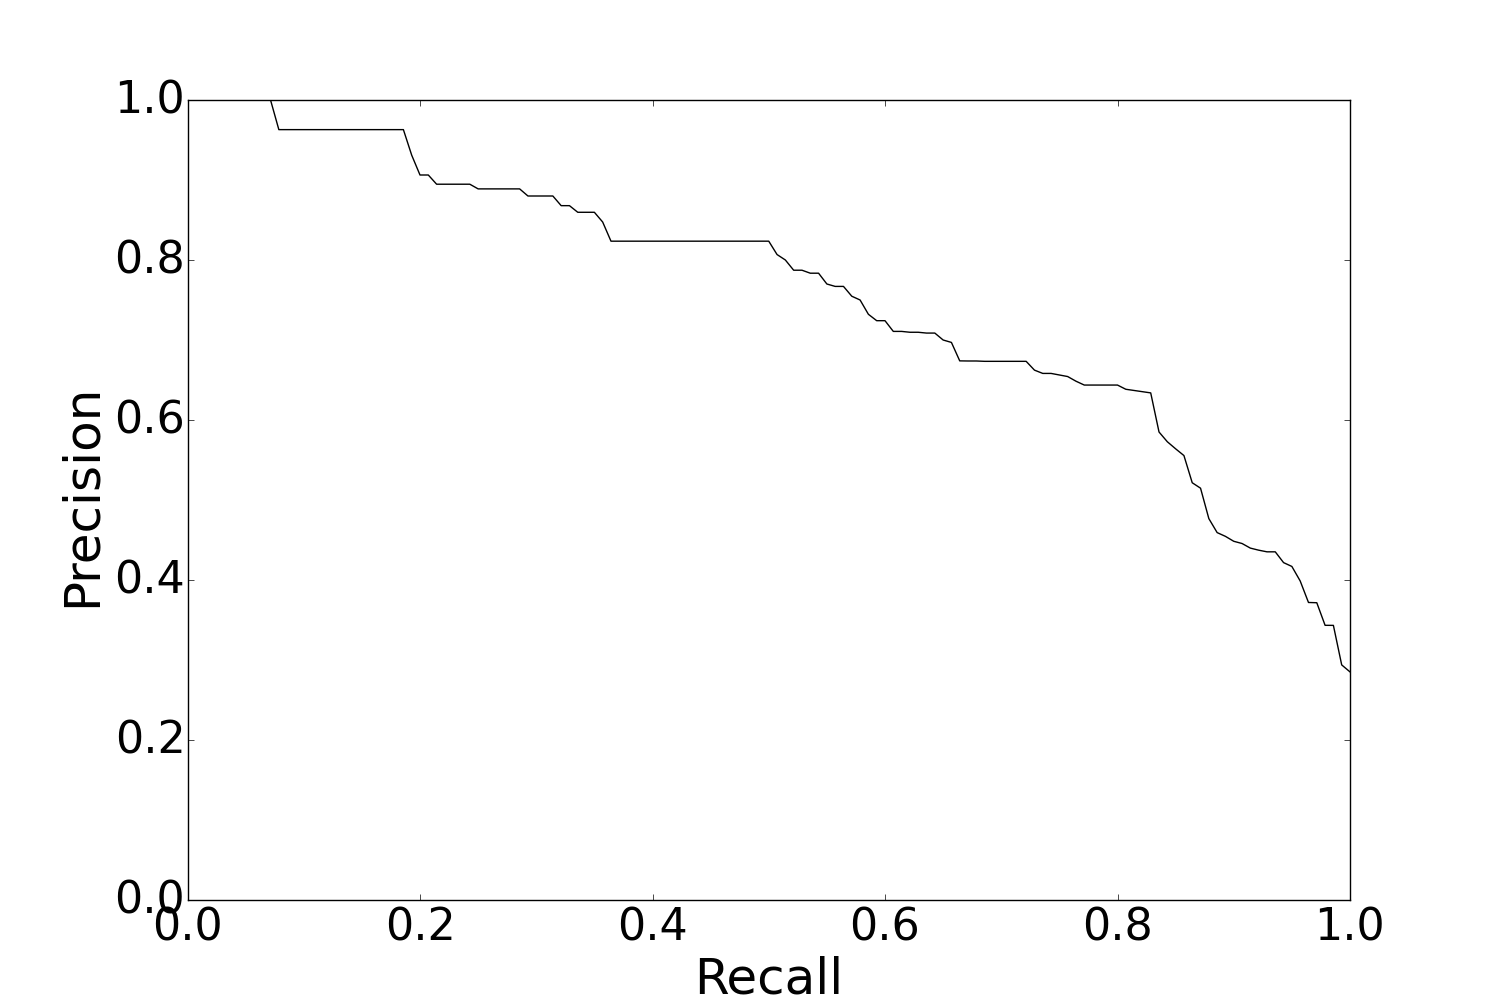
\includegraphics[scale=0.22]{pr/pr.png} 
\caption{Interpolated precision--recall curve for \textsc{ne-auto}.
\label{fig:pr}}
\end{center}
\end{figure}



%% \begin{table*}
%% \begin{center}
%% \begin{tabular}{lcccc}

%% \textbf{Method}& \textbf{Precision}&\textbf{Recall}
%% &\textbf{F1 score}&\textbf{Accuracy}\\
%%  \hline
%% Most-frequent class baseline & 0.498 & 0.497 & 0.498 & 0.663 \\

%% \hline

%% [A] Characater $n$-grams (1-3) & 0.665 & 0.576 & 0.615 & 0.787\\

%% [B] Character $n$-gram models & 0.399 & 0.499 & 0.443 & 0.787 \\

%% [C] Frequency & 0.395 & 0.500 & 0.441 & 0.789 \\

%% [D] Word embeddings & 0.803 & 0.773 & 0.787 & 0.863 \\

%% [E] Surface form & 0.792 & 0.573 & 0.660 & 0.813 \\ 

%% [A+B+C+D+E] & 0.814 & 0.761 & 0.786 & 0.865 \\

%% [B+C+D+E] & \textbf{0.817} & \textbf{0.787} & \textbf{0.801} & \textbf{0.872} \\

%% [A+C+D+E] & 0.820 & 0.758 & 0.787 & 0.866 \\

%% [A+B+D+E] & 0.810 & 0.757 & 0.782 & 0.864 \\

%% [A+B+C+E] & 0.676 & 0.597 & 0.633 & 0.792 \\

%% [A+B+C+D] & 0.813 & 0.756 & 0.783 & 0.864 \\
%% \end{tabular}
%% \caption{Macro-averaged precision, recall, and F1 score, as well as
%%   accuracy, for the baseline, each feature set, and combinations of
%%   features, using 2-way classification.\label{tbl:results}}
%% \end{center}
%% \end{table*}



\section{Conclusions}

In this paper we considered the problem of domain-specific OOV
classification in web forum text, focusing on the automotive
domain. We demonstrated that supervised methods trained on features
based on word embeddings for OOVs are highly informative for this
task, and can be complemented by information from features based on
linguistic knowledge of common properties of OOVs.  The coarse-grained
OOV categories that we predict could serve as a preliminary,
automatically-generated source of lexical knowledge about
OOVs. Moreover, we showed that such methods could be used to rank OOVs
to produce a semi-automated approach to identifying automotive named
entities among the OOVs.

In future work we intend to apply this approach to classifying OOVs to
build vocabularies focused on, or excluding, particular kinds of OOVs
to be used by other NLP applications, such as topic modeling. We
further intend to apply this knowledge in downstream NLP tasks, such
as named entity recognition, for domain-specific web forum text.

%% If accepted for publication, the final version of this paper would
%% include the following: 1.) an expanded discussion of the corpora used,
%% in particular further details of the web forum corpus; 2.) additional
%% discussion of the dataset of automotive OOVs, including further
%% details on the annotation process, OOV categories, and an
%% inter-annotator agreement study; 3.) additional word embedding
%% features incorporating embeddings for in-vocabulary terms for
%% categories such as \textsc{auto}, \textsc{ne-auto}, \textsc{ne-other},
%% and \textsc{slang}; 4.) an exploration of the impact of word2vec
%% parameter settings for building word embeddings from web forum text;
%% and 5.)  a more-detailed analysis of results, focusing in particular
%% on error analysis and per-class precision and recall.

\section{Acknowledgments}

This research is funded by the Natural Sciences and Engineering
Research Council of Canada.


% \nocite{*}
\section{Bibliographical References}
\label{main:ref}

\bibliographystyle{lrec2016}
\bibliography{local,../bibtex/big}


%% \section{Language Resource References}
%% \label{lr:ref}
%% \bibliographystylelanguageresource{lrec2016}
%% \bibliographylanguageresource{xample}

\end{document}
